% !TeX spellcheck = en_US

\chapter{Basis}
\label{chap:basis}

\section{Cloud Computing and Cloud application} \label{sec:cloud}

\subsection{Definitions}
Unfortunately, the is no generally accepted definition of cloud computing that describes all possible situations. 
But in scientific community the definition put forward by \textbf{N}ational \textbf{I}nstitute of \textbf{S}tandards and \textbf{T}echnology (NIST) is often used. 
This definition appropriately describes the concept of cloud computing used in this paper, and therefore this definition will be used and presented below.
\begin{definition}[Cloud computing]
	\label{def:nist}
Cloud computing is a model for enabling ubiquitous, convenient, on-demand network access to a shared
pool of configurable computing resources (e.g., networks, servers, storage, applications, and services) that
can be rapidly provisioned and released with minimal management effort or service provider interaction. \cite*{nist}
\end{definition}
Also the are no generally accepted definitions of cloud application, but it can be obtained from the definition of cloud computing.
\begin{definition}[Cloud application] 
	\label{def:capp}
	Cloud application is an application that is executed according to a cloud computing model. \cite*{cloudapp}
\end{definition} 
\subsubsection*{Service models}
NIST distinguishes between three types of service models.
\begin{itemize}
	\item Software as a Service (SaaS). 
	The capability provided to the consumer is to use the provider’s applications running on a cloud infrastructure. 
	The applications are accessible from various client devices through either a thin client interface, such as a web browser (e.g., web-based email), or a program interface. 
	The consumer does not manage or control the underlying cloud infrastructure including network, servers, operating systems, storage, or even individual application capabilities, with the possible exception of limited userspecific application configuration settings.
	\item Platform as a Service (PaaS). 
	The capability provided to the consumer is to deploy onto the cloud infrastructure consumer-created or acquired applications created using programming languages, libraries, services, and tools supported by the provider.
	The consumer does not manage or control the underlying cloud infrastructure including network, servers, operating systems, or storage, but has control over the deployed applications and possibly configuration settings for the application-hosting environment.
	\item Infrastructure as a Service (IaaS).
	The capability provided to the consumer is to provision processing, storage, networks, and other fundamental computing resources where the
	consumer is able to deploy and run arbitrary software, which can include operating systems and applications.
	The consumer does not manage or control the underlying cloud infrastructure but has control over operating systems, storage, and deployed applications; and possibly limited control of select networking components (e.g., host firewalls).
\end{itemize}

\subsubsection*{Deployment models}
Similarly, NIST distinguishes between four types of deployment models.
\begin{itemize}
	\item Private cloud. 
	The cloud infrastructure is provisioned for exclusive use by a single organization comprising multiple consumers (e.g., business units). It may be owned, managed, and operated by the organization, a third party, or some combination of them, and it may exist on or off premises.
\item Community cloud.
	The cloud infrastructure is provisioned for exclusive use by a specific community of consumers from organizations that have shared concerns (e.g., mission, security requirements, policy, and compliance considerations).
	It may be owned, managed, and operated by one or more of the organizations in the community, a third party, or some combination of them, and it may exist on or off premises.
\item Public cloud.
	The cloud infrastructure is provisioned for open use by the general public. 
	It may be owned, managed, and operated by a business, academic, or government organization, or some combination of them.
	It exists on the premises of the cloud provider.
\item Hybrid cloud. 
	The cloud infrastructure is a composition of two or more distinct cloud infrastructures (private, community, or public) that remain unique entities, but are bound together by standardized or proprietary technology that enables data and application portability (e.g., cloud bursting for load balancing between clouds). 
\end{itemize}

\subsection{Usage}
Now cloud computing and application can be found everywhere, and they number constantly grows. \cite*{cloud_stat}
They are used for test and development, big data analyses, file storage and so on.
Cloud computing allows you to effectively use resources, distributing the load to a system from several physical servers and shifting the maintenance to the providers. 
If your service uses a single one physical server and this server will be disabled, then entire service will be completely unavailable too.
But if you use cloud computing with a hundred of physical servers, then disabling one of them will not carry such serious consequences.
In addition, the user does not need to maintain a team of administrators for the event of various problems.\\
Usually the user does not have direct access to the infrastructure (servers and operating systems), he uses only provided interface.
An interface provides a set of methods to communicate with cloud infrastructure. 
Each provider defines his own set of methods, depending on his area of specialization. 
On the one hand this specialization makes it easier to work with the provider, on the other hand it becomes more difficult to switch to work with another provider.

\section{Topology and Orchestration Specification for Cloud	Applications (TOSCA)} \label{sec:tosca}
\subsection*{Definition}
The OASIS \cite{oasis} Topology and Orchestration Specification for Cloud Applications (\gls{tosca}) standard provides new ways to enable portable automated deployment and management of composite applications.
\gls{tosca} describes the structure of composite applications as topologies containing their components and their relationships.
Plans capture management tasks by orchestrating management operations exposed by the components. \cite*{INBOOK-2014-01}
\gls{tosca} application is a cloud application described according to TOSCA standard.
\subsection*{Usage}
\gls{tosca} can be used not only for describing all stages of a cloud application life-cycle, but alse serve as a layer between the cloud application and provider's interfaces, allowing to implement a single application suitable for working with different providers. 
\subsection*{Structure}
TOSCA specification provides a language to describe service components and their relationships using a service topology, and it provides for describing the management procedures that create or modify services using orchestration processes.
The combination of topology and orchestration in a Service Template describes what is needed to be preserved across deployments in different environments to enable interoperable deployment of cloud services and their management throughout the complete lifecycle (e.g. scaling, patching, monitoring, etc.) when the applications are ported over alternative cloud environments. \cite{TOSCA-v1.0_book} \\
Descriptions of the main components of \gls{tosca} used in this work will be provided.
\begin{itemize}
\item Service Template. 
	This component contains an Information about structure (TopologyTemplate) and Plans of cloud application.
\item Plans provides an interface to manage cloud application.
These components combine management capabilities to create higher-level management tasks, which can then be executed fully automated to deploy, configure, manage, and operate the application.
Plans are started by an external message and call management operations of the nodes in the topology.
\item Topology Template describes topology of cloud application, instantiating nodes (Node Templates) and relations between them (Relationship Templates).
\item Node Template specifies the occurrence of a Node Type as a component of a service.
\item Node Type defines the properties of such a component and the operations available to manipulate the component.
\item Relationship Template specifies the occurrence of a Relationship Type as a relationship between nodes in a Topology Template. 
	The Relationship Template indicates the elements it connects and the direction of the relationship by defining one source and one target element (in nested Source Element and Target Element elements).
\item Relationship Type defines the semantics and any properties of the relationship. \label{subs:reltype}
\item Artifact  represents the content needed to realize a deployment such as an executable (e.g. a script, an executable program, an image), a configuration file or data file, or something that might be needed so that another executable can run (e.g. a library).
	Artifacts can be of different types, for example EJBs or python scripts.
	The content of an artifact depends on its type. 
	Typically, descriptive metadata will also be provided along with the artifact.
	This metadata might be needed to properly process the artifact, for example by describing the appropriate execution environment.
	TOSCA distinguishes two kinds of artifacts: implementation artifacts and deployment artifacts.
\item Implementation Artifact represents the executable of an operation of a node type. An example will be provided in section \ref{sec:pm}
\item Deployment Artifact represents the executable for materializing instances of a node.
\item Artifact Type is describes an type of a artifact.
\item Artifact Templates represents information about the artifact. 
	Artifact location and other attendant data are stored here.
\item Node Type Implementation defines the artifacts needed for implementing the corresponding Node Type.
\end{itemize}
Types and Templates defining a TOSCA application are stored in definition documents.

\section{CSAR} \label{sec:csar}
A \textbf{C}loud \textbf{S}ervice \textbf{AR}chive (CSAR) is used to store the TOSCA application.
This is a ZIP-file with ".csar" extension that contains all the data needed for instantiation and management of TOSCA application.
These include definition documents, artifacts and so on.
In this form a TOSCA application can be processed by TOSCA runtime environment.
\subsection*{Structure}
The root folder must contain a "Definitions" and a "\gls{tosca}-Metadata" folders.
The "Definitions" folder contains definition documents, one of them must define Service Template.
The "\gls{tosca}-Metadata" folder must contain TOSCA metadata in form of file with the "TOSCA.meta" name.
This metafile consists of name/value pairs. 
One line for each pair. 
The first set of pairs describes CSAR itself (TOSCA version, CSAR version, creator and so on). 
All other pairs represent metadata of files in the CSAR

\subsection*{Terms}
Input \gls{csar} is a \gls{csar}, which can contain external references and will be processed by the framework.\\
Output CSAR is a SCAR, which was processed by the framework and doesn't contain external references.

\section{OpenTOSCA} \label{sec:opentosca}
OpenTOSCA provides an open source ecosystem for \gls{tosca} applications. 
The OpenTOSCA ecosystem consists out of three parts: \cite*{OpenTOSCA}
\begin{itemize}
	\item OpenTOSCA \textbf{Container}, a \gls{tosca} runtime environment
	\item \textbf{Winery} \label{tool:winery}, a graphical modelling TOSCA tool.
	\item \textbf{Vinothek}, a self-service portal for the applications available in the container
\end{itemize}
The runtime environment ant Winery will be provided in more details. 
\subsection*{Runtime environment}
The runtime enables fully automated plan-based deployment and management of applications in the CSAR format. 
First, the CSAR is unpacked and the files are put into the Files store.
Then, the TOSCA definitions documents are loaded, resolved, validated, and processed by the Control component, which calls the Implementation Artifact Engine and the Plan Engine.
The Implementation Artifact Engine deploys the referenced Implementation Artifacts and stores their endpoints in the Endpoints database. 
Finally, the Plan Engine binds and deploys the application’s management plans.
The endpoints of the management plans are stored in the Plans database.
\cite{INPROC-2013-45}
\subsection*{Winery}\label{subs:wine}
Winery works under the Tomcat runtime and therefore visual interface is available in browser, example in figure \ref{fig:winery_gui}.
Winery provides a complete set of functions for creating, editing and deleting all elements of the TOSCA topology. 
An example of TOSCA topology is presented on figure \ref{fig:winery_source}.
\begin{figure}[ht]   
	\centering
	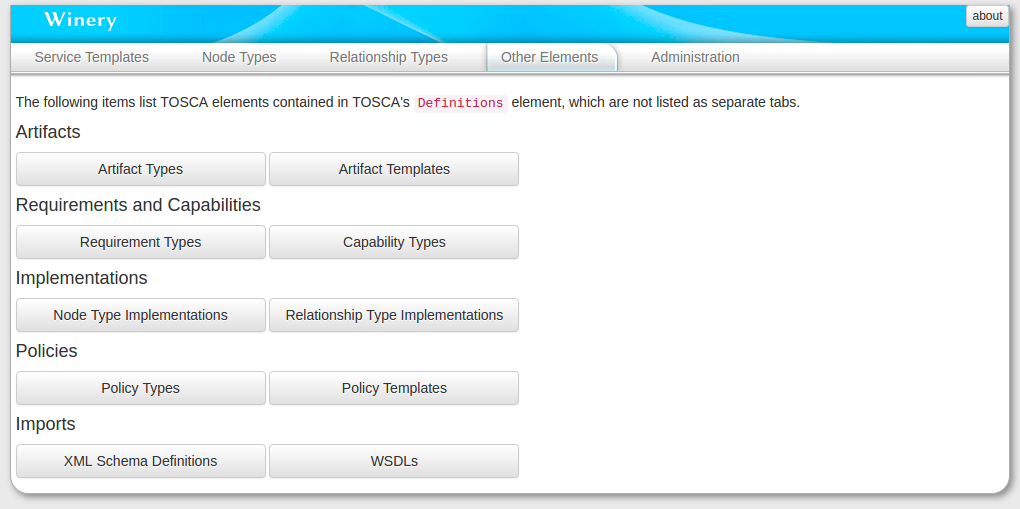
\includegraphics[width=0.7\textwidth]{Screenshot_winery_gui.png}
	\caption{Visual interface for $Winery$.}
	\label{fig:winery_gui}
\end{figure}
\begin{figure}[ht]   
\centering
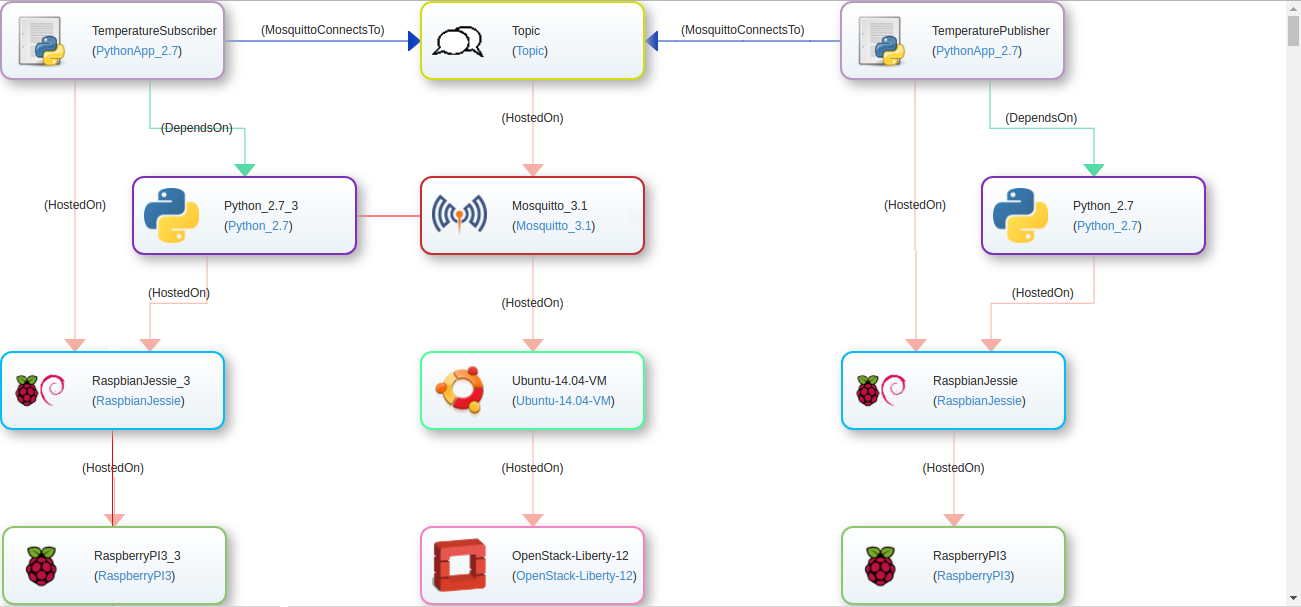
\includegraphics[width=0.7\textwidth]{Screenshot_winery_source.png}
\caption{TOSCA topology presented by $Winery$.}
\label{fig:winery_source}
\end{figure}

\section{Bash}
%TODO
\section{Ansible}
%TODO

\section{Package management} \label{sec:pm}
This section will describe the package management process and basic concepts from this area.
\subsection*{Package managers}
Package Manager is a set of software tools that automate the process of installing, updating, configuring and removing of computer programs.
A package can describe and contain not only a whole program, but also a certain component of a large application, hereinafter both will be referred as program components.
Package managers are used to manage the database of packages, their dependencies and versions, to prevent erroneous installation of programs and missing dependencies.
\subsection*{Packages}
A package is usually an archive containing both data for installation of the program component and a set of metadata like name, function, version, producer and dependencies.
\subsection*{Dynamic libraries}
Computer systems which rely on dynamic library linking, share executable libraries of machine instructions across packages and applications. 
In these systems, complex relationships between different packages requiring different versions of libraries results in a challenge colloquially known as "dependency hell".
Good package management is vital on these systems.
\subsection*{Repository}
To give users more control over the kinds of software that they are allowing to be installed on their system, software is often downloaded from a number of software repositories.
By default in Unix systems a package manager uses official repositories appropriate for the operating system and the device architecture, but the user can also additional repositories, like third-party repositories or repositories for another architecture.
\subsection*{Dependencies} \label{subs:dep}
Package managers distinguish between two types of dependencies: required and preRequired.
Dependency $package1$ $required$ $package2$ indicates that $package2$ must be installed for proper operation of $package1$.
Dependency $package1$ $preRequired$ $package2$ indicates that $package2$ must be installed for proper installation of $package1$.
An example of obtaining a dependency list is shown in listing \ref{lst:dep}.
\begin{lstlisting}[caption={Example of using $apt$-$cache$ to obtain dependency list for package python}\label{lst:dep},captionpos=t] 
user@user:~$ apt-cache depends python
python
PreDepends: python-minimal
Depends: python2.7
Depends: libpython-stdlib
Conflicts: <python-central>
Breaks: update-manager-core
Suggests: python-doc
Suggests: python-tk
Replaces: python-dev
\end{lstlisting}
%TODO add example dependencies output
\subsection*{Dependency tree}
In the example above $package2$ is needed for $package1$, but $package2$ itself can require additional packages.
A structure describing all needed packages and dependencies between them for given root-package is called a dependency tree. 
Dependency type $required$ leads to the presence of cycles in dependency tree, which differs them from normal tree graph structures.


